%!TeX root=../tese.tex

%%%%%%%%%%%%%%%%%%%%%%%%%%%%%%%%%%%%%%%%%%%%%%%%%%%%%%%%%%%%%%%%%%%%%%%%%%%%%%%%

\chapter{Fundamentos e Trabalhos Relacionados}%
\label{cha:fundamentos_e_trabalhos_relacionados}

\section{Detecção de Sarcasmo}%
\label{sec:deteccao_de_sarcasmo}

De acordo com o dicionário Dicio, \textbf{sarcasmo} é uma zombaria que busca
ofender, enquanto \textbf{ironia} é a ação de dizer o oposto do que se deseja
expressar. Ainda segundo ele, a diferença entre esses dois termos se dá no fato
de que sarcasmo é um dito ácido que pode ou não ser expresso por meio de uma
ironia e essa, por sua vez, pode ou não ser utilizada para
ofender.~\cite{dicio_sarc, dicio_irony}

O termo \textbf{detecção de sarcasmo} refere-se à determinação de se há ou não
sarcasmo em uma porção de texto verbal. E o termo \textbf{detecção automática de
sarcasmo} refere-se a resolução (ou tentativa de) resolver o problema mencionado
utilizando métodos computacionais que automatizam essa decisão.
Computacionalmente, podemos definir esse problema como uma \textbf{classificação
binária} de texto, termo explicado mais a frente.

Entretanto, na literatura é bastante comum também se definir detecção de
sarcasmo como a determinação de se há ou não sarcasmo ou ironia verbal em uma
porção de texto verbal. Portanto, em geral, ao se falar de sarcasmo, a
literatura engloba tanto sarcasmo quanto ironia como se fossem a mesma coisa.
Este texto também não fará discriminação entre sarcasmo ou ironia.

Em geral, esse problema é difícil, pois, por vezes, nem humanos conseguem
perceber essa figura de linguagem (e.g. ``\textit{Oba, hoje está tão ensolarado,
que vontade de ir para a escola.}''). Além disso, o contexto tende a importar
muito. Muitas características externas ao texto podem servir para descriminar se
uma pessoa está ou não sendo sarcástica. Entre alguns exemplos estão intonação,
locutor, interlocutor, conhecimento prévio sobre a fala, tempo e espaço em que
se fala e elementos não verbais.~\cite{wallace-etal:2014:ironic-context}

\section{Classificação binárias}%
\label{sec:classificacao_binarias}

O problema de detecção de sarcasmo pode ser tratado como uma classificação
binária. Esse tipo de problema é muito estudado no campo do aprendizado de
máquina e envolve classificar os elementos de um conjunto em dois grupos
chamados de classes. Por classificar entende-se a determinação de um elemento do
conjunto entre pertencente à primeira ou segunda classe.

No caso da detecção de sarcasmo, os elementos são os pedaços de texto e as duas
classes são \textit{ser sarcástico} e \textit{não ser sarcástico}. Em termos
matemáticos, tem-se um conjunto de exemplos denotado pela matriz $X$ de
dimensões $n\times m$, onde $n$ é o número de exemplos e $m$ é o número de
características que se usa para descrever cada um desses exemplos. Cada linha de
$X$ é denotada por $\xii[x]{i}$ e chamada de \textit{exemplo} $i$ ou
\textit{instância} $i$.

A linha $\xii[x]{i}$ é um vetor de $m$ posições em que cada posição é uma
característica que descreve a entrada. Por exemplo, na detecção de sarcasmo, o
primeiro valor pode ser a quantidade de palavras, o segundo valor pode ser a
quantidade de caracteres, a terceira pode ser a soma de positividade do texto
(definida por algum critério específico) e assim por diante. É importante que a
mesma posição em diferentes instâncias tenha o mesmo significado. Portanto, caso
se defina que a primeira posição represente o número de palavras, todas as
instâncias devem seguir essa regra.

Cada instância $i$ pertence ou à primeira classe ou à segunda, modela-se isso
por um valor $\xii[y]{i}$ chamado de $i$-ésimo rótulo (do inglês,
\textit{label}). E escreve-se $\xii[y]{i}\in\set{0, 1}$, onde cada valor
representa uma das classes. No caso de sarcasmo, pode-se representar por
\textit{não sarcasmo} o valor $0$ e \textit{sarcasmo}, o valor $1$. Com esses
valores $\xii[y]{i}$ constrói-se um vetor $y$ onde $y_i=\xii[y]{i}$.

Ao final, o problema é descobrir uma função $f$ que mapeie bem $X$ em $y$. Note,
entretanto, que $n$, o número de exemplos, é possivelmente infinito, pois sempre
se pode achar novos exemplos e testar se $f$ os mapeia corretamente. Portanto,
na prática, o valor de $n$ é limitado às instâncias em um determinado
\textit{conjunto de dados} coletado de alguma forma (manual, semi-automática ou
automática). Ou seja, tenta-se achar essa função $f$ conhecendo parcialmente o
conjunto das instâncias. Além disso, após encontrar a função $f$ nesse conjunto
limitado de dados, chamado de \textit{dados de treinamento}, deseja-se
utiliza-la para discriminar novos textos similares aos originais, mas para os
quais não se sabe de antemão se são ou não sarcásticos. Esses novos dados são,
em muitos casos, chamados de \textit{dados de teste}.

Vale a pena, entretanto, mencionar que os dados de treinamento geralmente são
divididos em duas ou três partições que são chamadas de \textit{dados de
treinamento}, \textit{dados de validação} e \textit{dados de teste}. Essa
nomenclatura pode ser um pouco confusa, pois os termos acabam se repetindo.
Portanto, daqui em diante se utilizará \textit{dados rotulados} para os dados
que se sabe a classe de antemão (ou seja, sabe-se se aquele texto é ou não
sarcástico) e \textit{dados não rotulados} para os dados novos em que se deseja
aplicar $f$ e não se sabe a classe de antemão.

\subsection{Métricas de avaliação}%
\label{sub:metricas_de_avaliacao}

Para saber se a função $f$ mapeia bem $X$ em $y$, é preciso definir uma
\textbf{métrica de avaliação}, que é uma função matemática bem definida que
indica quanto de erro se comete em determinado conjunto finito de exemplos $X$.

Dado um conjunto de entrada $X$ com $n$ instâncias, seja $y$ o vetor que
representa se cada instância é ou não sarcástica. Seja então $f$ a função sob
avaliação (ou seja, a função de modelagem que recebe os textos e determina se
são ou não sarcásticos). Seja $\hat{y}=f(X)$ os resultados gerados por essa
função.

Note que para cada exemplo $i$, podemos ter duas opções:

\begin{center}
\begin{tabular}{ c c }
  $\hat{y}_i=y_i$ & \textit{acerto} \\
  $\hat{y}_i\neq y_i$ & \textit{erro}
\end{tabular}
\end{center}

Além disso, note que o par $\pair{y_i}{\hat{y}_i}$ pode ter quatro valores:

\begin{table}[h]
  \centering
  \caption{Os nomes dados para os diferentes tipos de erros e acertos.}
  \label{tab:tabela_casos_error_acerto}
  \begin{tabular}{ c | c c c }
    $\pair{y_i}{\hat{y}_i}$ & caso & nome em inglês & notação \\
    \hline
    $\pair{1}{1}$ & verdadeiro positivo & \textit{true positive} & $tp$
    \\
    $\pair{0}{1}$ & falso positivo & \textit{false positive} & $fp$
    \\
    $\pair{0}{0}$ & verdadeiro negativo & \textit{true negative} & $tn$
    \\
    $\pair{1}{0}$ & falso negativo & \textit{false negative} & $fn$
  \end{tabular}
\end{table}

Nesses quatro casos, dois correspondem a quando o modelo acerta, os verdadeiros
positivos e verdadeiros negativos, e dois correspondem a erros, os falsos
positivos e falsos negativos. Os falsos positivos são, em alguns contextos,
chamados de erros tipo 1, e são cometidos quando uma instância é erroneamente
classificada como positiva. Já os falsos negativos são também chamados de erros
tipo 2, e são cometidos quando uma instância é erroneamente classificada como
negativa.

Com esses valores em mente, pode-se definir algumas métricas que ajudam a
perceber quão boa a função $f$ é. Dessa forma, pode-se comparar duas funções
$f$.

\paragraph{Acurácia}%
\label{par:acuracia}

Definida simplesmente como a quantidade total de acertos divido pela quantidade
total de instâncias. Seja $n'$ a quantidade de acertos, então:
\[
\texttt{Acurácia} = \dfrac{n'}{n}
\]

É comum também definir a acurácia em termos dos valores acima listados:
\[
\texttt{Acurácia} = \dfrac{tp+tn}{tp+tn+fp+fn}
\]

Note que $tp+tn$ representa justamente quando $\hat{y}_i=y_i$ e $fp+fn$,
representa quando $\hat{y}_i\neq y_i$.

\paragraph{Precisão}%
\label{par:precisao}

Definida como:
\[
\texttt{Precisão} = \dfrac{tp}{tp+fp}
\]

é a taxa de verdadeiros positivos em relação todas as instâncias preditas como
positivas. Portanto, é a fração entre todas as instâncias previstas como
positivas e as instâncias que realmente eram positivas. Ela pune o modelo quando
ele comete erros do tipo 1, ou seja, quando classifica valores demais como
positivos.

\paragraph{Revocação}%
\label{par:revocacao}

Muitas vezes chamada por seu nome em inglês, \textit{recall}, é definida como:
\[
\texttt{Revocação} = \dfrac{tp}{tp+fn}
\]

é a taxa de verdadeiros positivos em relação a todos os positivos. Portanto,
mede a fração de quantos positivos foram acertados em relação a todos os que
existiam no conjunto observado. Ela pune o modelo quando ele comete erros do
tipo 2, ou seja, quando ele deixa de classificar um valor como positivo.

A precisão e a revocação guardam uma relação chave entre si e geralmente se quer
ter um bom balanço entre as duas. Note que o modelo deve achar um ponto ótimo
entre classificar valores como $1$ demais (baixa precisão) e de menos (baixa
revocação). Observe essa relação a partir do seguinte exemplo.

Comece com a função
\begin{equation}
  f\paren{\xii[x]{i}} = 1~~\forall i
\end{equation}

Como ela sempre considera a entrada como positiva, então os únicos casos
existentes serão de verdadeiros e falsos positivos. Logo:
\[
\texttt{Precisão} = \dfrac{tp}{tp+fp} = \dfrac{tp}{n}
\]
e
\[
\texttt{Revocação} = \dfrac{tp}{tp+fn} = \dfrac{tp}{tp+0} = 1
\]

Portanto, a revocação terá o maior valor possível, enquanto a precisão será
exatamente a fração de valores positivos que o conjunto observado possui. Como,
semanticamente, a revocação é penalizada sempre que um elemento é positivo, mas
foi previsto como negativo, então faz sentido que se tenha uma revocação de
$100\%$, já que não se comete esse tipo de erro.

Agora, tome a função
\begin{equation}
  f\paren{\xii[x]{i}} = 0~~\forall i
\end{equation}

Como ela sempre considera a entrada como negativa, então os únicos casos
existentes serão de verdadeiros e falsos negativos. Logo:
\[
\texttt{Precisão} = \dfrac{tp}{tp+fp} = \dfrac{0}{0+fp} = 0
\]
e
\[
\texttt{Revocação} = \dfrac{tp}{tp+fn} = \dfrac{0}{0+fn} = 0
\]

Portanto, como a função nunca tenta marcar uma instância como positiva, ela
nunca acerta os verdadeiros positivos e comete $100\%$ de erro.

\begin{figure}[h]
\centering
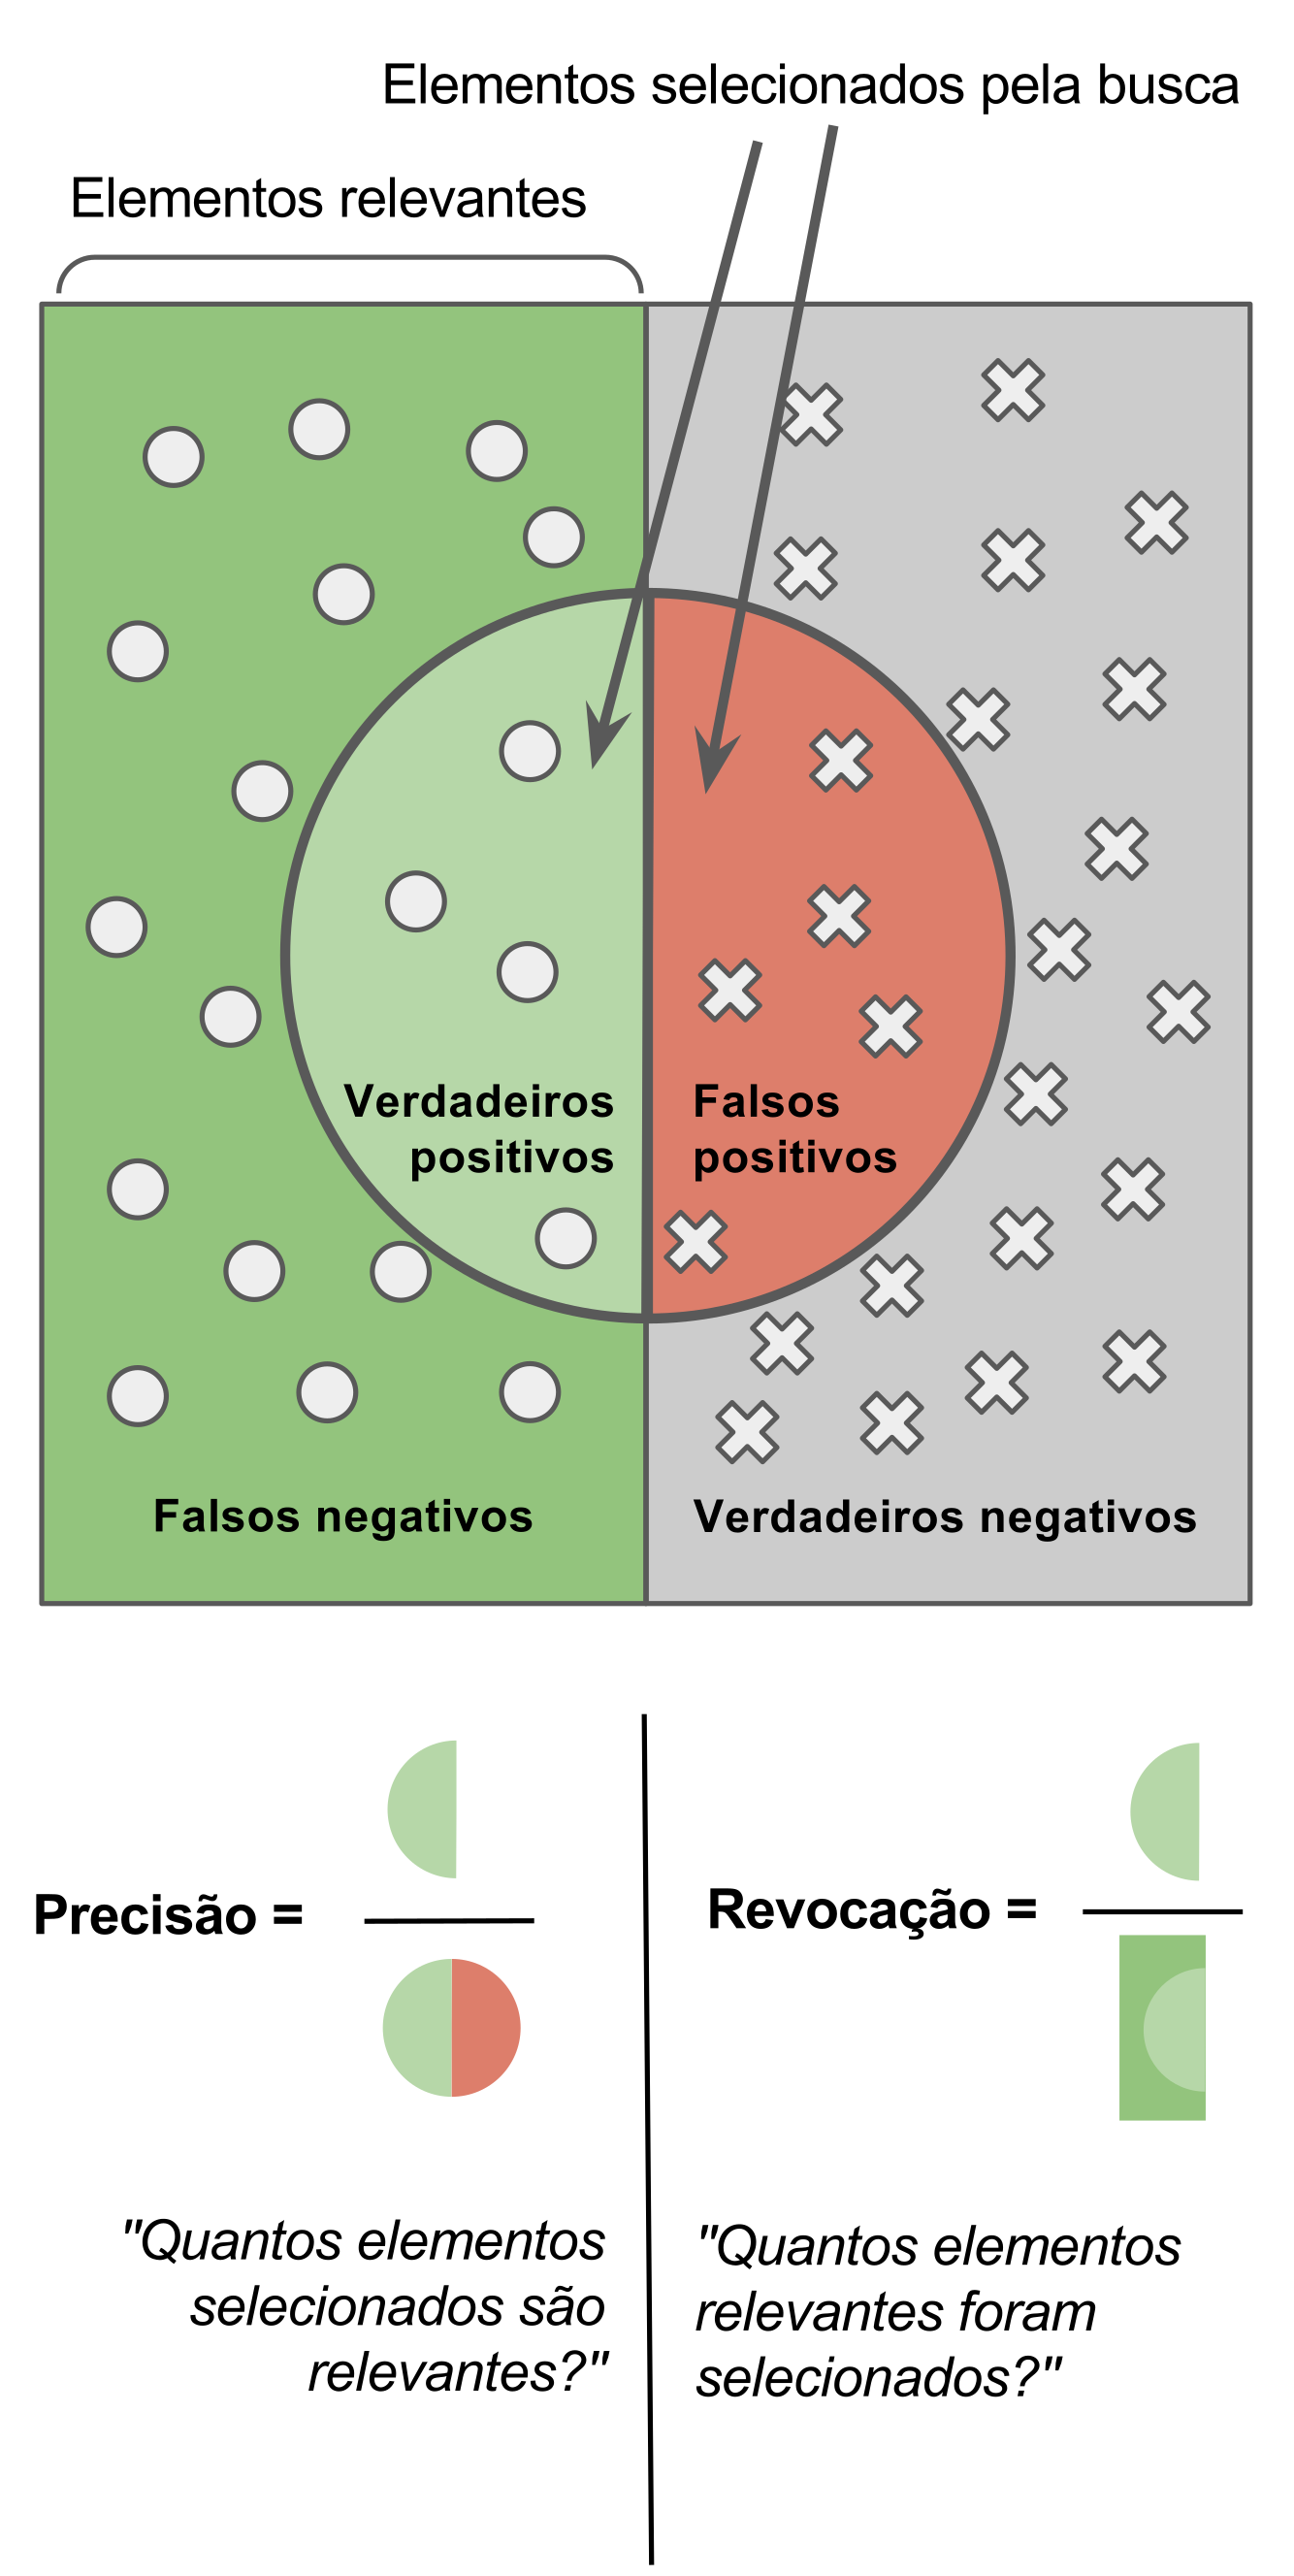
\includegraphics[scale=1]{Res/precision_recall.png}
\caption{Imagem ilustrando os conceitos de precisão e revocação. No centro,
estão os elementos preditos como positivos ($\hat{y_i}=1$). Na esquerda
(representados por círculos), estão os elementos verdadeiros ($y_i=1$). Na
direita (representados por cruzes), estão os elementos falsos ($y_i=0$). Imagem
retirada de \cite{bernadofbbraga:2017:precisao_revocacao}.}
\label{precision_recall.png}
\end{figure}

\paragraph{Métrica $F_1$}%
\label{par:metrica_f_1_}

Por esses e outros motivos, é interessante agregar a precisão e revocação em um
único valor, que permite fácil comparação entre dois modelos. É possível
utilizar uma média simples desses dois valores, mas é muito mais comum a
utilização da métrica $F_1$ (ou, do inglês, $F_1$ \textit{score}).

Ela é definida como:
\[
F_1=2\cdot
\dfrac{\texttt{precisão}\cdot\texttt{revocação}}
{\texttt{precisão}+\texttt{revocação}}
\]

Obter um valor $F_1$ alto significa que ambas precisão e revocação são altas.

\section{Trabalhos Relacionados}%
\label{sec:trabalhos_relacionados}

Esta seção aborda os trabalhos e as diferentes abordagens realizados na área.
Pode-se caracterizar os trabalhos por três principais tipos de abordagens: as
baseadas em regras, baseadas em métodos de aprendizado e baseadas em contexto.
Além disso, fala-se um pouco sobre as principais características extraídas dos
textos que são utilizadas para melhorar a eficácia das soluções.

\subsection{Abordagens Baseadas em Regras}%
\label{sub:abordagens_baseados_em_regras}

Abordagens baseadas em regras são aquelas que usam regras fixas para determinar
se uma sequência de palavras contém ou não ironia. Para criar essas regras,
várias características do texto podem ser utilizadas, como as classes sintáticas
das palavras, se são palavras de cunho positivo ou negativo, se há a presença ou
não de certas palavras em uma ordem, entre qualquer outro tipo de regra
proposta.

Essa abordagem é computacional, porque as regras formam um algoritmo que pode
ser implementado por uma linguagem de computação. Dessa forma, qualquer
sequência de palavras pode ser dada como entrada para o algoritmo e ele
retornará se ele acredita que essa sequência contém ou não sarcasmo.

A principal vantagem desse tipo de abordagem é que ela, além de detectar o
sarcasmo, ajuda a estudá-lo. Ao criar uma regra do tipo \textit{se o texto
possui essas características, então ele é sarcástico} se cria uma explicação
para as principais características presentes em um texto sarcástico.

Entretanto, as metodologias utilizadas são bastante específicas para cada tipo
de texto e cada conjunto de dados. As regras criadas para um determinado
conjunto, por exemplo, da rede social Twitter podem não funcionar em outras
redes sociais como o Facebook, o Instagram ou o WhatsApp, pois cada uma dessas
redes sociais possui um contexto e formato de conversação muito diferente.
Portanto, são modelos que nos permitem explicar o processo de decisão, mas não
permitem fácil generalização.

\cite{veale:2010} investigam em seu artigo sequências da forma ``\textit{as * as
a *''} (``tão * quanto um(a) *''), consideradas como analogias entre o que os
autores chamam de \textit{base} (\textit{ground}) e \textit{meio}
(\textit{vehicle}). Eles utilizam a API do Google para coletar 45021 instâncias
do padrão ``\textit{about as * as *}'' e filtram os resultados manualmente para
chegar em 20299 instâncias que de fato são consideradas analogias. Eles então
anotam manualmente os rótulos para essas instâncias e encontraram que 15502
casos ($76\%$) são irônicos e apenas 4797 ($24\%$) são não irônicos.

Então, dado uma sequência ``\textit{as * as a *}'', os autores utilizam
mecanismos de busca na rede como a API do Google para distinguir entre três
casos: os casos em que essa sequência nunca foi usada como ``\textit{about}'';
aqueles que já foram, mas não frequentemente; e aqueles que são frequentemente
usados com essa marcação. Segundo os próprios autores, essas três categorias
fornecem, respectivamente, evidencia fraca contra ironia, evidencia fraca a
favor da ironia e evidência forte para ironia. Ou seja, o caso em que se tem
mais certeza de que é uma ironia é o caso em que a sequência é frequentemente
utilizada junto com a palavra ``\textit{about}''.

Assim sendo, \cite{veale:2010} criam uma sequência de nove passos para
classificar uma frase desse tipo entre as classes \textit{ironia} e \textit{não
ironia}. Esses passos são bastante claros e precisos, podendo ser, portanto,
implementados por um programa de computador e caracterizando, por conseguinte,
uma detecção automática de sarcasmo.

Nessas regras, os autores utilizam o fato de que analogias mais frequentemente
utilizadas são menos prováveis de serem irônicas, pois a ironia utiliza bastante
a criatividade do locutor para fazer analogias não usuais.

Devido à natureza das regras propostas pelos autores, eles conseguem medir a
precisão e revocação obtidas por cada uma das regras. No geral, o modelo atinge
uma acurácia de $88\%$, o que é um valor bastante alto para esse tipo de
problema. Entretanto, note que os autores se limitaram a um escopo muito fechado
(das frases do tipo ``\textit{as * as a *}'').

\cite{maynard-greenwood:2014:cares} exploram o uso de regras baseadas em
\textit{hashtags} presentes em postagens da rede social Twitter e sua aplicação
para detecção de sarcasmo em um contexto mais geral de análise de sentimento.

Em seu artigo, eles utilizam um algoritmo de tokenização de \textit{hashtags}
para transformá-las em palavras com as quais eles conseguem extrair informação.
No caso, eles utilizam as palavras contidas nas \textit{hashtags} para avaliar
se o sentimento é positivo ou negativo e inverter o sentido original da frase
caso detectem sarcasmo nas \textit{hashtags}. Por exemplo, a \textit{hashtag}
\textit{\#notreally} é tokenizada em \textit{not} e \textit{really} e
identificada como uma \textit{tag} sarcástica de acordo com regras definidas
pelos autores.

Então, eles aplicam cinco regras que podem determinar o sentimento de uma
postagem como \textit{negativo} ou \textit{positivo}, ou então trocar o
sentimento pré-determinado da postagem. Os autores, assim, fazem uso da detecção
de sarcasmo utilizando \textit{hashtags} para resolver um outro problema mais
geral que é definir o sentimento predominante de um texto.

Como ponto negativo de sua técnica, está o fato de que nem sempre o tokenizador
de \textit{hashtags} funciona de forma adequada. Por exemplo,
\textit{\#greatstart} pode ser dividida de duas formas: \textit{greats} e
\textit{tart} ou \textit{great} e \textit{start}. Um ser humano provavelmente
saberia que a segunda opção é a mais provável, mas o algoritmo não sabe fazer
essa distinção e acaba ficando com o primeiro conjunto e palavras. Apesar disso,
esse sistema de tokenização possui um $F1$ de $97,25\%$ e os autores obtiveram
$91\%$ de precisão e revocação na tarefa no conjunto de dados utilizado por
eles.

\cite{bharti-etal:2015:parsing-sarcasm} apresentam duas abordagens baseadas em
regras. A primeira é através da análise morfossintática (do inglês,
\textit{Part-of-Speech Tagging}) e criação de árvores sintáticas (do inglês,
\textit{parse-trees}) que identificam a positividade do sentimento e situação
predominantes em \textit{tweets}. A segunda é através da análise sintática de
\textit{tweets} que começam com interjeições.

Em sua primeira abordagem, os autores utilizam dicionários e algoritmos
pré-criados para encontrar as classes morfológicas e sintáticas das palavras.
Então, baseando-se nisso, utilizam um algoritmo criado por eles para
encontrar um valor de positividade para o sentimento do texto e para a situação
retratada e, caso seus valores tenham sinais contrários (sentimento positivo e
situação negativa ou vice-versa), eles consideram o texto como sarcástico. Por
exemplo, em ``\textit{I hate Australia in cricket, because they always win}''
(``eu odeio a Australia no críquete, porque eles sempre ganham''), as palavras
``\textit{I hate}'' apresentam um sentimento negativo, enquanto as palavras
``\textit{they always win}'' retratam uma situação positiva, e, portanto, essa
frase seria classificada como sarcástica em sua primeira abordagem.

Em sua segunda abordagem, os autores utilizam novamente algoritmos de
\textit{POS Tagging} pré-criados para achar as classes morfológicas e sintáticas
de palavras em \textit{tweets} que começam com interjeições, como \textit{wow},
\textit{oh}, \textit{wow}, \textit{aha}, \textit{yay}, \textit{yeah},
\textit{nah}, etc. Em seu algoritmo, eles classificam como sarcásticos os textos
que começam por interjeições e possuem um adjetivo ou advérbio imediatamente
após a interjeição, ou então possuem, em alguma posição após a interjeição, ou um
advérbio seguido de adjetivo ou um adjetivo seguido de um substantivo ou um
advérbio seguido de um verbo. Essa abordagem é bastante interessante, pois ela é
bastante simples e, ainda assim, consegue um ótimo resultado de 0.90 $F_1$ no
subconjunto de \textit{tweets} marcado com a hashtag \textit{sarcasm}.

\subsection{Conjuntos de Características}%
\label{sub:conjuntos-de-caracteristicas}

Antes de prosseguir com as abordagens, essa seção mostra um pouco dos
principais conjuntos de características usados. Abordagens
baseadas em regras utilizam determinadas características como principalmente as
classes morfossintáticas das palavras. Entretanto, as abordagens listadas a
seguir fazem uso de conjuntos muito maiores de características retiradas do
texto e vários trabalhos foram realizados para expandir a quantidade de
características possíveis de se utilizar.

Como dito anteriormente, ao criar a matriz de exemplos de entrada $X$, cada
coluna representa uma característica do texto. Dessa forma, o texto fica
agregado em um conjunto de valores numéricos que são acessíveis para a máquina
utilizar e comparar. Ao invés de se comparar dois texto distintos com números de
caracteres e palavras diferentes, utiliza-se um algoritmo para extrair
características (do inglês, \textit{features}) comuns entre os textos e
compará-los por meio dessas características.

Um exemplo é o método chamado \textit{bag-of-words} (em tradução literal,
``sacola-de-palavras'') que cria um vetor com, por exemplo, 512 posições de
valores naturais onde cada posição do vetor representa quantas vezes uma
determinada palavra  apareceu no texto. Cada posição do vetor é associada a uma
palavra e, muitas vezes, utiliza-se uma outra posição especial para denotar
qualquer palavra que não está no dicionário de palavras selecionadas
previamente. Por exemplo, a primeira posição pode representar quantas vezes a
palavra ``\textit{a}'' aparece no texto, a segunda posição pode representar
quantas vezes a palavra ``\textit{the}'' aparece, e assim por diante. Se a
palavra ``Lucas'' for lida, então será adicionado um à última posição do vetor,
que é utilizado para contar qualquer palavra que não é uma das outras 511.

\begin{figure}[h]
\centering
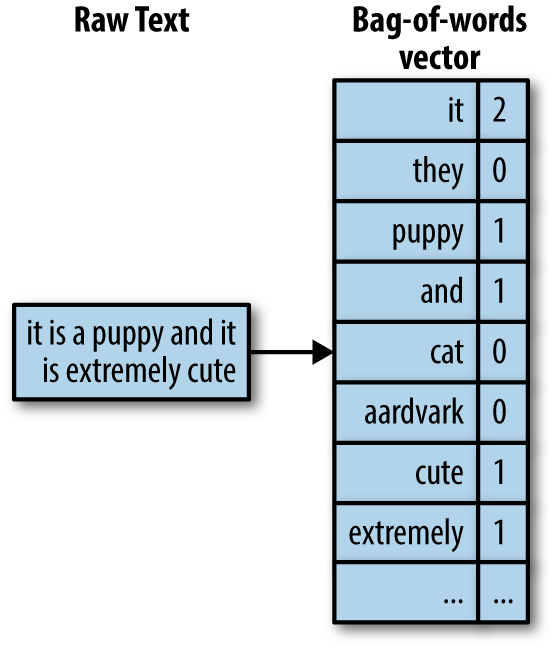
\includegraphics[scale=1.3]{Res/bow-image.png}
\caption{Na esquerda, o texto e na direita o vetor criado pelo algoritmo
\textit{bag-of-words} para representar o texto. Imagem retirada de
\cite{zheng-casari:2018:feature-engineering}.}
\label{bow-image.png}
\end{figure}



\cite{reyes:2012:from-humor} exploram quatro grupos de características dentro de
um contexto mais geral de detecção de humor e ironia. Esses grupos são:
ambiguidade, através dos níveis estrutural, morfossintático e semântico;
polaridade, através de palavras que possuam semântica positiva ou negativa;
imprevisibilidade, através de desbalanceamentos contextuais entre o significado
literal das palavras; e os cenários emocionais, através das emoções passadas por
cada palavras.

\cite{liebrecht:2013:perfect-solution} utilizam uni-, bi- e trigramas como
características do texto. Um n-grama é uma sequência de n palavras do texto.
Portanto, nesse tipo de característica, o unigrama seria o \textit{bag-of-words}
clássico citado acima, com as contagens de cada palavra, já o bigrama se trata
das contagens de duas palavras seguidas. Por exemplo, sempre que as palavras
``\textit{so nice}'' aparecerem em sequência, adiciona-se um à coluna que se
refere a essa sequência.

\cite{reyes:2013:multidimensional-approach} utilizam uma abordagem parecida com
\cite{reyes:2012:from-humor}, com quatro grupos de características: assinaturas,
imprevisibilidade, estilo e cenários emocionais. Cada um dos grupos foca em
várias características. Dentro das assinaturas, por exemplo, há o foco em
pontuações específicas, emojis, citações e palavras em maiúsculas; há o foco em
marcas implícitas que geram oposição entre partes do texto; e há o foco na
compressão temporal, que identifica oposição temporal entre elementos
relacionados.

A grande diferença desse trabalho em relação aos demais está, entretanto, no
grupo de características de estilo. Esse grupo tenta modelar o estilo de escrita
do texto para, assim, fazer a diferenciação entre estilos sarcásticos e não
sarcásticos. Para fazer isso, eles utilizam três tipos de sequências textuais:
n-gramas no nível de caracteres (ao invés de palavras) (abreviado pelos autores
por \textit{c-grams}), \textit{skip-grams} (\textit{s-grams}) e
\textit{skip-grams} de polaridade (\textit{ps-grams}).

Os \textit{c-grams} capturam a frequência de sequências de informação
morfológica como sufixos e prefixos (como \textit{-ly}, \textit{-ing},
\textit{dis-}, \textit{un-}). Os \textit{s-grams} funcionam como n-gramas, mas
com alguns pulos entre palavras e são utilizados para obter relações entre
palavras não adjacentes no texto. Por exemplo, na sentença ``Hoje está chovendo,
quero tanto ir à praia'', um bigrama é representado pela sequência ``Hoje
está'', enquanto um bigrama com pulo de uma palavra seria ``Hoje chovendo''. Por
fim, os \textit{ps-grams} criam uma sequência de rótulos de positividade baseado
nos \textit{s-grams}. Por exemplo, ``Hoje chovendo'' seria rotulado como
``pos-neg'' (positivo e negativo).

\cite{barbieri:2014:modelling-sarcasm}, por sua vez, criar um dos conjuntos mais
completos de características, com setes grupos. Esses grupos são: frequência,
que mede o quão comum é cada palavra utilizada no texto; escrito-falado (da
tradução literal de \textit{written-spoken}, utilizado pelos autores em seu
artigo), que funciona como a frequência, mas a frequência que a palavra é usada
em diálogos escritos em oposição a falados; intensidade, que mede o uso de
adjetivos e advérbios para aumentar ou diminuir a intensidade semântica de
outras palavras no texto; estrutura, que mede, por exemplo, o número de
caracteres usados, o número de palavras, o tamanho médio das palavras, o número
de verbos, de substantivos, o número total de pontuações, o número de risadas, o
número de vírgulas, pontos finais, sinais de exclamação, o número de emojis (ou
emoticons), o número de organizações, pessoas, títulos e datas citados pelos
texto; sentimento, que mede valores de positividade entre as palavras e usa
algumas métricas como soma dos valores positivos, soma dos negativos, média da
diferença entre positivos e negativos, entre outros; sinônimos, que calcula
métricas relacionadas aos sinônimos das palavras usadas no texto, como a
quantidade de sinônimos que uma determinada palavra tem e que possuem frequência
de utilização menor do que ela; e ambiguidade, que mede a quantidade de sentidos
possíveis que uma palavra pode ter.

\cite{joshi:2015:context-incongruity} propõem uma nova abordagem baseada em uma
teoria linguística chamada de incongruência de contexto. Eles se baseiam no fato
de que o tempo para um ser humano processar um texto sarcástico depende do grau
de incongruência presente nele e criam características o que chamam de
incongruências explícitas e implícitas. A primeira é caracterizada por palavras
de sentimentos opostos e a segunda é caracterizada por frases de sentimento
implícito, que não se pode detectar através de uma única palavra.

\cite{mishra:2016:harnessing-cognitive} seguem por uma abordagem bastante
diferente das demais, que utiliza características baseadas no movimento
produzido pelos olhos de pessoas lendo textos sarcásticos. Algumas das
características propostas por eles são a fixação da visão em pontos do texto e
saltos mais rápidos entre duas porções do texto do que em relação às demais.
Além disso, eles utilizam um grafo de informação estrutural ao utilizar as
palavras como vértices do grafo e os saltos de visão entre as palavras como
arestas.

\subsection{Abordagens Baseadas em Métodos de Aprendizado}%
\label{sub:abordagens_baseadas_em_metodos_de_aprendizado}

Métodos de aprendizado são aqueles que usam modelos baseados em aprendizado de
máquina. Dentro desse campo do conhecimento, existem alguns tipos de
aprendizado. Dentre eles, os principais são o \textbf{aprendizado
supervisionado}, o \textbf{aprendizado semi-supervisionado}, o
\textbf{aprendizado não supervisionado} e o \textbf{aprendizado por reforço}.
Pesquisadores já fizeram uso dos três primeiros tipos de aprendizados listados,
mas nesta monografia ater-se-á apenas aos trabalhos envolvendo aprendizado
supervisionado, pois são os mais similares às técnicas aqui utilizadas. Para uma
listagem mais vasta dos trabalhos correlacionados, recomenda-se a leitura dos
trabalhos de \cite{joshi:2017:sarcasm-detection-survey} e
\cite{yaghoobian:2021:sarcasm-detection-comparative-study}.

Dentro do campos do algoritmos de aprendizado supervisionado estão os algoritmos
de classificação, que como dito anteriormente, trata-se de achar uma função $f$
que mapeie bem os exemplos $X$ em seus respectivos rótulos $y$. A matriz $X$
contém diversas características extraídas do texto, como as exploradas em
\ref{sub:conjuntos-de-caracteristicas}. E o vetor de rótulos $y$ contém números
associados às classes de classificação. No caso da classificação binária, são
apenas duas classes (que, em detecção de sarcasmo, são \textit{sarcasmo} e
\textit{não sarcasmo}), mas em contextos mais gerais, podem haver várias
classes, como em análise de sentimento. Nesse caso, as classes podem ser o
sentimento predominante no texto e sarcasmo é apenas mais uma entre outras
classes. Isso depende de como cada autor quer modelar o problema e quais
aplicações se espera ter de resultado.

Em abordagens clássicas utilizando aprendizado de máquina, muitos trabalhos se
baseiam em modelos bem conhecidos e estudados como \textit{decision trees} (DT),
\textit{random forecasts} (RF), \textit{support vector machines} (SVM),
\textit{naive Bayes} (NB) e \textit{Neural Networks}
(NN)~(\cite{yaghoobian:2021:sarcasm-detection-comparative-study}). Esses modelos
são utilizados em várias áreas nas quais se aplica o aprendizado de máquina e
são aplicados por muitos autores sem colocar seu foco principal em modificar o
modelo ou criar modelos específicos para a detecção de sarcasmo. Em alguns
outros trabalhos, entretanto, os autores procuram alternativas menos conhecidas
ou modelos híbridos para conseguir melhores resultados.

\cite{riloff:2013:sarcasm-constract} utilizam uma abordagem híbrida que combina
as previsões de uma SVM com um método baseado em contraste. Dessa forma, os
autores combinam uma abordagem baseada em aprendizado com uma baseada em regras
para criar um novo modelo. Nesse modelo, sempre que qualquer uma das duas
abordagens classificar o texto como sarcástico, então o texto é classificado
como sarcástico pelo modelo final.

\cite{liebrecht:2013:perfect-solution} fazem uso de um algoritmo menos conhecido
chamado de \textit{balanced winnow}, que é similar ao algoritmo
\textit{perceptron}. Esse algoritmo permite a investigação de quais
características foram mais importantes para fazer a classificação.  Dessa forma,
é possível procurar quais os padrões mais importantes para o classificador e
tentar entender por que esse é o caso.

Similarmente, árvores de decisão (do inglês \textit{decision trees}) foram
experimentadas por \cite{reyes:2013:multidimensional-approach} para poder
investigar a ordem de decisões tomadas pela árvore para ver também quais
características fazem a maior diferença e explicam mais o resultado. Além disso,
eles usam também o modelo \textit{naive Bayes}, pois seu artigo utiliza diversas
características booleanas (com valores zero ou um).

\cite{joshi-etal:2016:harnessing} partem para um estudo e abordagem diferentes.
Ao invés de utilizar bases de dados de redes sociais, como o frequentemente
utilizado Twitter, eles exploram a detecção de sarcasmo em diálogos da séries de
TV ``\textit{Friends}''. E argumentam que o problema de detecção de sarcasmo de
diálogos é melhor modelado como uma tarefa de rotulação de sequências ao invés
de uma tarefa de classificação de cada rótulo isoladamente.

Nessa modelagem, a ordem em que as falas de um diálogo aparecem é levada em
conta. Ao invés de tomar uma fala isoladamente e classificá-la, o modelo deve
classificá-la utilizando todas as falas que vieram antes dela. Eles, então,
utilizam dois modelos de aprendizado de máquina, o SEARN e o SVM-HMM e mostram
que esses modelos de sequência performam melhor que os classificadores
tradicionais.

\cite{liu-etal:2014:imbalanced-classification} apresentam uma nova estratégia
chamada por eles de \textit{multi-strategy ensemble learning approach} (MSELA).
Em seu trabalho, eles exploram a detecção de sarcasmo em um conjunto de dados
bastante desbalanceado (ou seja, com uma proporção pequena de textos sarcásticos
em relação aos não sarcásticos). Para lidar com esse problema, eles propõem essa
estratégia.

A MSELA é constituída de três partes diferentes. A primeira é chamada de
\textit{sample-ensemble strategy} (em tradução livre, ``estratégia de conjunto
de amostragens'') e consiste em fazer amostragens nos dados originais de forma a
criar $N$ conjuntos da dados balanceados. Cada um desses sub-conjuntos de dados
é então usado para treinar pequenos classificadores, que consistem da segunda
parte: a \textit{classifier-ensemble strategy} (em tradução livre, ``estratégia
de conjunto de classificadores''). Nessa etapa, cada os classificadores de cada
sub-conjunto de dados não necessariamente são os mesmos. Os autores empregam
três tipos de classificadores (sendo que, em teoria, pode-se utilizar mais) e,
para cada sub-conjunto, escolhem um classificador aleatório para ser treinado.
Por fim, a terceira etapa serve para juntar cada uma das classificações em uma
única e é chamada de \textit{weighted voting strategy} (em tradução livre,
``estratégia de voto ponderado''). Nessa última estratégia, as decisões de cada
classificador são ponderadas por uma medida de entropia da informação e, dessa
forma, unidas para resultar em uma última decisão de se o texto é ou não
sarcástico.

Além do modelos de aprendizado tidos como mais ``clássicos'', modelos de
aprendizado profundo (ou seja, aqueles que utilizam grandes redes neurais)
também foram utilizados. Esse tipo de modelo costuma resultar em melhores
métricas, mas também exige uma quantidade muito grande de dados. Isso por muitas
vezes é um problema, pois a maioria dos conjuntos de dados é rotulado por seres
humanos que decidem se um texto é ou não sarcástico utilizando seus próprios
conhecimentos.

\cite{ghosh-veale:2016:fracking-sarcasm-nn} utilizam três tipos de redes neurais
em conjunto e comparam seu desempenho em um conjunto de dados extraído do
Twitter. Eles utilizam \textit{long short-term memories} (LSTMs),
\textit{convolutional neural networks} (CNNs) e \textit{deep neural networks}
(DNNs), combinando esses modelos entre si para conseguir melhores resultados.

\cite{van-hee-etal:2018:semeval} mostram em seu artigo os resultados da terceira
tarefa da SemEval-2018, um \textit{workshop} internacional de PLN com o objetivo
de avançar as fronteiras do estado-da-arte em determinadas tarefas. Nesse
artigo, eles mostram que as melhores soluções (em termos da métrica $F_1$)
propostas pelos times utilizam modelos baseados em aprendizado profundo. Eles
fazem principalmente o uso de redes do tipo LSTMs, CNNs e DNNs. Além disso, é
presente o uso de \textit{word embeddings} como o GloVe, que retratam cada uma
das palavras presentes em um texto como vetores reais nos quais palavras de
sentidos parecidos possuem vetores parecidos.

A tarefa proposta pela SemEval-2018 era dividida em duas sub-tarefas. A primeira
era uma detecção de sarcasmo comum, onde bastava o modelo distinguir entre
\textit{tweets} sarcásticos e não sarcásticos. A segunda tarefa, entretanto, era
mais complexa, pois exigia que o modelo também classificasse o tipo de sarcasmo
que ocorria no texto. Os resultados mostraram que mesmo modelos de aprendizado
profundo bastante sofisticados ainda estavam bastante longe de resultados
promissores. Enquanto na primeira sub-tarefa o melhor time obteve uma métrica
$F_1$ de $0.705$, o melhor time na segunda sub-tarefa obteve apenas $0.507$
pontos dessa mesma métrica.

\subsection{Abordagens Baseadas em Contexto}%
\label{sub:abordagens_baseadas_em_contexto}

Até então, foram exibidos trabalhos que se restringem apenas ao texto de
interesse. Entretanto, muitos outros trabalhos partem de outra abordagem, que é
utilizar informações além do texto para se determinar se um texto é ou não
sarcástico, chamadas de contexto.

\cite{wallace-etal:2014:ironic-context} mostram em seu artigo que humanos obtém
melhores resultados para detectar se um texto é ou não sarcástico quando eles
recebem contexto além do texto original. Em seu trabalho, eles exploram a rede
social Reddit e pedem para seres humanos decidirem se uma postagem nessa rede é
ou não sarcástica e qual o seu grau de confiança nessa decisão. O humano pode
pedir por contexto quando estiver em dúvida e os autores, então, apresentam qual
era o tópico em que a postagem estava inserida e uma lista de outras postagens
do mesmo usuário.

Eles então mostram que serem humanos acertam consistentemente mais quando obtém
esse contexto extra, além de ficarem mais confiantes em sua decisão. Não só
isso, mas os autores também mostram que um modelo \textit{bag-of-words} costuma
errar nesses casos em que humanos precisam de contexto extra. Portanto, os
autores argumentam que máquinas provavelmente também precisam de contexto extra
para conseguir melhores resultados. Nos anos seguintes, muitos outros autores
criaram modelos que utilizam o contexto de uma postagem e provam empiricamente
que o contexto pode ajudar.

Há muitas formas de se adicionar informações extras referentes ao contexto.
\cite{hazarika-etal:2018:cascade} criam um método para criar representar
\textit{embeddings} de usuários, que capturam o estilo de descrita e
personalidade para criar uma representação que pode ser utilizada em adição ao
texto escrito por aquele usuário.

\cite{kolchinski-potts:2018:representing-social-media-users} exploram outra
forma de se criar \textit{embeddings} para os usuário de uma rede social. Para
cada autor nos dados de treinamento, ele criam um vetor de 15 valores
randômicos. Então esses vetores são passados como entrada para um modelo de rede
neural recorrente (RNN) bidirecional e são atualizados durante o treinamento,
com o objetivo de aprender características importantes do usuário. Então se
aquele usuário aparece novamente na hora de fazer uma predição fora dos dados de
treinamento, seu vetor de \textit{embeddings} é utilizado. Contudo, caso o autor
não tenha aparecido no treinamento, um vetor randômico é utilizado.

\cite{wang-etal:2015:context-twitter} utilizam o contexto da conversa e do
tópico, utilizando os \textit{tweets} que vieram antes do \textit{tweet} de
interesse, outros \textit{tweets} do mesmo autor e outros \textit{tweets} que
tenham as mesmas \textit{hashtags} do \textit{tweet} de interesse (ou seja, que
pertençam ao mesmo tópico).

O melhor resultado obtido por eles é quando utilizam o histórico de
\textit{tweets} do autor. Eles experimentam com o último \textit{tweet} do
autor, os três últimos e os cinco últimos, obtendo melhores resultados conforme
aumentavam esse número. Além disso, utilizar o contexto da conversa (ou seja, o
histórico de respostas de que levou até o \textit{tweet} de interesse) possui
também um ganho nas métricas, mas variar entre 1, 3 ou 5 \textit{tweets} não
muda muito. Isso mostra que se o modelo tivesse acesso apenas ao \textit{tweet}
de interesse (que queremos determinar sarcasmo) e o \textit{tweet} que ele
respondeu (o anterior a ele na conversa) já teria a maior parte do ganho que
se obteria ao olhar para a conversa toda. Intuitivamente, isso faz sentido, pois
quando se dá uma resposta sarcástica, essa é uma resposta àquilo que foi falado
imediatamente antes na vasta maioria dos casos. Por fim, eles mostram que a
métrica $F_1$ cai ao adicionar contexto do tópico e que, portanto, adicionar
outros \textit{tweets} com a mesma \textit{hashtag} do de interesse apenas
atrapalha.

\cite{ghosh:2018:sarcasm-conversation-context} também utilizam contexto da
conversa em conjunto com LSTMs e mostram que ao adicionar a postagem que foi
respondida pela postagem de interesse melhora os resultados. Eles utilizam
vários conjuntos de dados e várias formas diferentes de LSTMs, assim, eles
testam diversas maneiras de se acoplar o comentário anterior ao de interesse e
mostram que adicionar o contexto referente à postagem anterior sempre melhora os
resultados.

\cite{jena-etal:2020:cnet} criam um novo modelo chamado por eles de C-Net que
foca também em utilizar o contexto gerado pelos comentários anteriores de um
comentário de interesse. Dado que eles tenham $n-1$ comentários anteriores, eles
criam $n$ modelos BERT, um para cada comentário. Assim, em uma cadeia de $n$
comentários (onde o $n$-ésimo é o comentário de interesse, o $n-1$-ésimo é o
comentário anterior a ele e assim por diante), o $i$-ésimo BERT é treinado
utilizando apenas o $i$-ésimo comentário e deve retornar uma porcentagem $y_i$
de que o comentário $i$ leve a uma resposta sarcástica. Depois, eles agregam
esses resultados dos $n$ modelos utilizando uma camada de fusão (do inglês,
\textit{fusion layer}) que utiliza algum modelo que recebe $n$ valores e retorna
uma probabilidade final $y_{n+1}$ que será utilizada para dizer se o último
comentário foi ou não sarcástico. Para fazer essa concatenação, eles utilizam
um modelo de séries temporais chamado de \textit{simple exponential smoothing}
(SES).

Por fim, há outras duas formas de se adicionar contexto à tarefa. A primeira
delas é utilizando \textit{word embeddings}, pois elas permitem aos modelos que
as utilizam fazer comparações entre palavras e compreender a semântica passada
por elas. Alguns exemplos são
\texttt{Word2vec}~(\cite{mikolov-etal:2013:word2vec}),
\texttt{GloVe}~(\cite{pennington-etal:2014:glove}),
\texttt{fastText}~(\cite{bojanowski-etal:2016:fasttext}),
\texttt{ELMo}~(\cite{peters-etal:2018:elmo}),
\texttt{BERT}~(\cite{devlin-etal:2018:bert}).
A segunda é pelo uso de uma técnica chamada de transferência de aprendizado (ou
aprendizado por transferência) (do inglês, \textit{transfer learning}),
que consiste de um modelo treinado em tarefas genéricas utilizando um conjunto
de dados realmente grande. Esse modelo passa a ser chamado de
\textbf{pré-treinado} e seus parâmetros são salvos para serem refinados (do
inglês, \textit{fine-tuning}) depois em uma tarefa específica.  Dentro do
contexto de PLN, os modelos mais utilizados são os conhecidos como
\textit{transformers} (explicados em
\ref{sec:modelos_de_redes_neurais_transformers}).
Alguns exemplos são
\texttt{GPT-3}~(\cite{brown-etal:2020:gpt3}),
\texttt{XLNet}~(\cite{yang-etal:2019:xlnet}),
\texttt{BERT}~(\cite{devlin-etal:2018:bert}),
\texttt{RoBERTa}~(\cite{liu-etal:2019:roberta})
e \texttt{DeBERTa}~(\cite{he-etal:2020:deberta}), que é o foco deste trabalho.

Entre os trabalhos que utilizam \textit{transformers}, um dos mais bem sucedidos
é o de \cite{potamias-etal:2020:transform-sarcasm}, que criam um modelo que
utiliza um RoBERTa em conjunto com uma LSTM bidirecional (BiLSTM). Os autores
argumentam que o RoBERTa é capaz de mapear as palavras para um espaço vetorial
rico em semântica e que outros modelos de redes neurais podem usar esses valores
para capturar dependências tempo-espaciais entre as palavras. Eles, portanto,
removem a última camada do modelo pré-treinado RoBERTa e passam os valores da
sua última camada escondida (do inglês, \textit{hidden layer}) para uma BiLSTM
que, por sua vez, tem seus resultados concatenados por uma camada completamente
conectada e passados para uma camada \textit{softmax}.

\section{Modelos de Redes Neurais \textit{Transformers}}%
\label{sec:modelos_de_redes_neurais_transformers}

A proposta desse trabalho é aplicar um tipo de \textit{transformer} chamado de
DeBERTa~(\cite{he-etal:2020:deberta}) e comparar seu resultado com outros
\textit{transformers}, que hoje constituem o estado-da-arte em muitas tarefas de
PLN (entre elas, a detecção de
sarcasmo)~(\cite{joshi:2017:sarcasm-detection-survey}).  Essa seção tem por
objetivo apresentar em maiores detalhes o funcionamento desse tipo de
arquitetura de redes neurais (NN) e apresentar os \textit{transformers} mais
conhecidos e utilizados.

\subsection{RNNs}%
\label{sub:rnns}

Para se chegar em como os \textit{transformers} foram criados, é interessante
dar um panorama histórico do estado-da-arte no processamento de linguagem
natural e, em especial, na tarefa de tradução automática. Devido à
característica sequencial de qualquer texto, redes neurais recorrentes (RNNs)
são a principal escolha para esse tipo de tarefa.

Uma RNN é uma rede neural que consiste de um estado escondido (do inglês,
\textit{hidden state}) $h$ e uma saída opcional $y$ que recebe como entrada uma
sequência de tamanho variável $x=\paren{\seq{x}{T_x}}$. A cada passo temporal
$t$, o estado escondido $h_t$ da RNN é atualizado pela função $f$:

\begin{equation}
h_t = f\paren{h_{t-1}, x_t},
\label{eq:rnn}
\end{equation}

onde $f$ é uma função de ativação não linear que pode ser tão simples quando uma
sigmoide ou tão complexa quanto uma unidade \textit{long short-term memory}
(LSTM), introduzida por \cite{hochreiter-schmidhuber:1997:lstm} em 1997.

A RNN, então, consegue aprender uma distribuição de probabilidade com base na
sequência de entrada ao ser treinada para predizer o próximo elemento da
sequência. Portanto, ao receber uma sequência $x=\paren{\seq{x}''{t-1}}$, ela
consegue retornar a probabilidade do próximo elemento da sequência ser $j$ ao
utilizar uma função de ativação do tipo \textit{softmax} em sua saída:

\begin{equation}
  p\paren{x_{t,j}=1 \cond \seq{x}{t-1}} =
  \dfrac{\exp \paren{w_j h_t}}
  {\spsum{j'=1}{K}\exp\paren{w_{j'}h_t}},
\end{equation}

onde $w_j$ é a $j$-ésima linha de uma matriz de pesos $W$.

\begin{figure}[h]
\centering
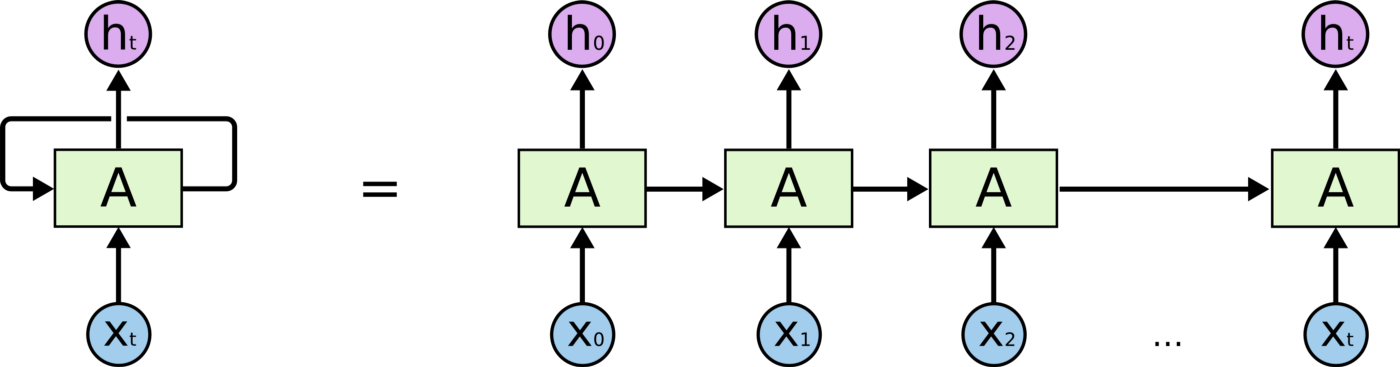
\includegraphics[scale=0.24]{Res/rnn.png}
\caption{Imagem representativa de uma RNN. Na esquerda a representação compacta
e na direita a representação expandida. Imagem retirada de
\cite{radhakrishnan:2017:introduction-rnn}.}
\label{rnn.png}
\end{figure}

Utilizando esse tipo de rede neural, \cite{cho-etal:2014:rnn-encoder-decoder}
propõem uma nova arquitetura chamada de \textit{RNN Encoder-Decoder}, que
utiliza uma RNN para codificar a sequência de entrada $x$ em um único vetor $c$
de dimensão pré-definida chamado de \textbf{contexto} (não confundir com
contexto já mencionado em \ref{sub:abordagens_baseadas_em_contexto}), que, por
sua vez, é passado como entrada para uma segunda etapa de decodificação, que
produz uma nova sequência $y$. No caso de tradução de texto, a sequência $x$ é o
texto a ser traduzido e a sequência $y$ é o texto após tradução.

\begin{figure}[h]
\centering
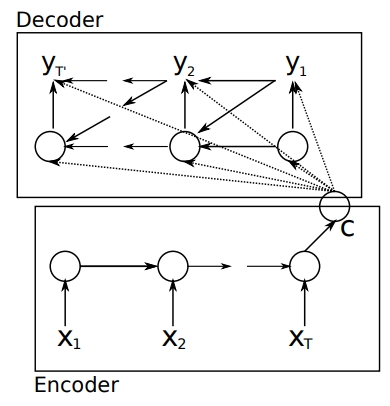
\includegraphics[scale=0.6]{Res/rnn-ed.jpg}
\caption{Representação de uma \textit{RNN Encoder-Decoder}. Imagem retirada de
\cite{cho-etal:2014:rnn-encoder-decoder}.}
\label{rnn-ed.jpg}
\end{figure}

Diferentemente de \ref{eq:rnn}, o estado escondido do decodificador, $s_t$, não
é uma função da entrada, mas sim do contexto gerado pelo codificador e também
pelo último elemento da saída produzido:

\begin{equation}
s_t = f\paren{s_{t-1}, y_{t-1}, c},
\label{rnn-decoder}
\end{equation}

e o próximo elemento da saída é gerado utilizando a função de distribuição dada
por:

\begin{equation}
P(y_t\cond\seq{y}{t-1},c)=g\paren{y_{t-1},s_t,c},
\end{equation}

onde $f$ e $g$ são funções de ativações e $g$ deve ser uma função que produz
probabilidades válidas (como, por exemplo a \textit{softmax}). Vale ainda
ressaltar que para escolher $y_t$, o próximo elemento da sequência de saída do
modelo, pode-se utilizar várias estratégias. As mais conhecidas são escolher
$y_t$ como o elemento de maior probabilidade da função de distribuição ou então
escolher um elemento aleatoriamente ponderando pelas probabilidades de cada
elemento (isto é, elementos com valores de probabilidade mais altos dados pela
distribuição têm maiores chances de serem escolhidos como o próximo elemento da
sequência de saída).

\subsection{Mecanismos de Atenção}%
\label{sub:mecanismos_de_atencao}

\cite{bahdanau-etal:2014:attention-mechanism} estendem a arquitetura de
\cite{cho-etal:2014:rnn-encoder-decoder} criando um mecanismo que mais tarde
ficaria conhecido como \textbf{mecanismo de atenção}.

Primeiramente, eles o fato de que o vetor $c$ é fixo em todas as iterações de
cálculo do novo estado escondido. Cada $s_i$ é uma função de um vetor de
contexto $c_i$:

\begin{equation}
  s_i=f\paren{s_{i-1},y_{i-1},c_i}.
\end{equation}

O vetor de contexto, por sua vez, é criado como sendo uma combinação linear dos
estados gerados pelo codificador, $\set{\seq{h}{T_x}}$, ponderado por valores
$\alpha_{ij}$:

\begin{equation}
  c_i=\spsum{j=1}{T_x}\alpha_{ij}h_j
  \label{eq:attention}
\end{equation}

Os valores $\alpha_{ij}$ são calculados de maneira que formem uma distribuição
de probabilidades. Ou seja, cada valor $\alpha_{ij}$ está entre zero e um e a
sua soma em $j$ vale um. Isso é garantido ao utilizar a função \textit{softmax}:

\begin{equation}
  \alpha_{ij}=\dfrac{\exp\paren{e_{ij}}}
  {\spsum{k=1}{T_x}\exp\paren{e_{ik}}},
\end{equation}

onde

\begin{equation}
  e_{ij}=a\paren{s_{i-1},h_j}.
\end{equation}

A função $a$ por sua vez é uma função que retorna uma pontuação para quanta
atenção o modelo deve prestar ao redor da posição $j$ da entrada para predizer a
posição $i$ da saída. No artigo original de
\cite{bahdanau-etal:2014:attention-mechanism} é utilizada uma rede completamente
conectada que é treinada juntamente com o restante do modelo.

Para resumir antes de prosseguir, o codificador itera sobre os valores da
sequência de entrada $x=\paren{\seq{x}{T_x}}$ e gera uma sequência
$h=\paren{\seq{h}{X_T}}$ que representa aquela entrada, mas codificada através
da equação \ref{eq:rnn}\footnote{No artigo original, os autores na verdade
utilizam uma BiRNN, mas por propósitos didáticos, isso foi abstraído.}.

Na arquitetura comum de um \textit{encoder-decoder}, os valores de $h$ são
utilizados diretamente para gerar a saída. Entretanto,
\cite{bahdanau-etal:2014:attention-mechanism} propõem que exista uma camada
intermediária entre o codificador e decodificador que faz com que o
decodificador foque sua atenção (intuitivamente falando) em elementos
específicos da sequência $h$. Para tanto, o $i$-ésimo contexto, $c_i$, que
gera a $i$-ésima saída $y_i$, é criado através de uma soma que percorre cada
elemento $h_j$ e o multiplica por uma probabilidade $\alpha_{ij}$ de $h_j$ ser
relevante na predição de $y_i$.

Após essa nova proposta de \cite{bahdanau-etal:2014:attention-mechanism}, muito
são os trabalhos que utilizam, adaptam e incrementam o mecanismo de atenção.
\cite{galassi:2021:attention-in-nlp} fazem uma revisão de diversos mecanismos de
atenção utilizados na literatura e propõem um modelo genérico que engloba grande
parte dos trabalhos que fazem uso desse mecanismo.

\begin{figure}[h]
\centering
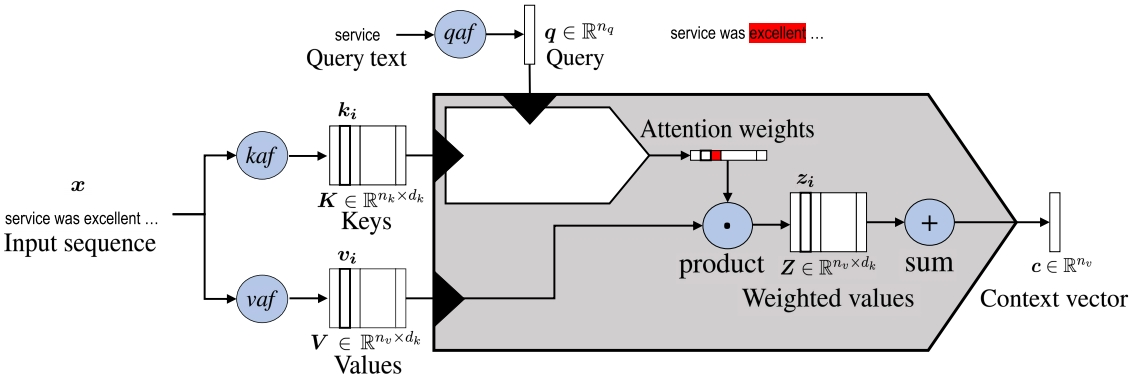
\includegraphics[scale=0.5]{Res/attention-img1.jpg}
\caption{Um modelo geral de mecanismos de atenção. Imagem retirada de
\cite{galassi:2021:attention-in-nlp}.}
\label{attention-img1.jpg}
\end{figure}

\subsection{\textit{Transformers}}%
\label{sub:transformers}

Mecanismos de atenção são utilizados em conjunto a uma RNN, de maneira similar a
\cite{bahdanau-etal:2014:attention-mechanism}, por muitos outros trabalhos.
RNNs, entretanto, possuem um problema intrínseco em sua arquitetura, que é o
fato de serem recorrentes. Isso significa que uma RNN precisa do valor do estado
escondido anterior $h_{t-1}$ para calcular o novo estado $h_t$ (seja no
codificador ou decodificador). Dessa forma, não se pode paralelizar sua
computação facilmente. \cite{vaswani-etal:2017:attention-is-all-you-need} criam,
então, um novo modelo chamado de \textit{transformer}~\footnote{o termo
\textit{transformer} é uma palavra em inglês que significa ``transformador'',
mas nesta monografia opta-se por utilizar o próprio termo em inglês
\textit{transformer}}.

Essa nova arquitetura se baseia apenas em uma versão nova do mecanismo de
atenção para criar um modelo do tipo \textit{encoder-decoder}, que pode ser
aplicado sobre uma sequência, de forma análoga a uma RNN. Esse novo modelo de
atenção é chamado de \textit{self-attention} (em tradução literal,
``\textit{atenção a si próprio}'').

Nele, todos os elementos da sequência de entrada podem ser processados ao mesmo
tempo pelo codificador e os de saída pelo decodificador.  Entretanto, suponha
que se quer prever o elemento $y_i$ da sequência de saída.  Nesse caso, o
\textit{transformer} recebera a sequência $x$ e a sequência correta de saída
$y$, mas os elementos $y_j$ com $j\geq i$ são mascarados para simular uma RNN,
que não tem acesso a esses valores (e também limitar a trivialidade que seria
predizer o elemento $y_i$ com esse elemento dado como entrada para o modelo).

Para dar um exemplo, suponha que a tarefa é de tradução do português para o
inglês e que se deseja traduzir a frase ``Atenção é tudo que você precisa'' para
a frase ``\textit{Attention is all you need}''. Portanto, tem-se
$x=\paren{\texttt{Atenção}, \texttt{é}, \texttt{tudo}, \texttt{que},
\texttt{você}, \texttt{precisa}}$ e $y=\paren{\textit{Attention}, \textit{is},
\textit{all}, \textit{you}, \textit{need}}$. Em caso de se desejar prever o
terceiro elemento da sequência, $y_3$, o valor de entrada é a própria sequência
$x$, mas a entrada da saída gerada até agora é $y=\paren{\textit{Attention},
\textit{is}, \texttt{<MASK>}, \texttt{<MASK>}, \texttt{<MASK>}}$, onde
$\texttt{<MASK>}$ é um token especial que acaba recebendo uma atenção de menos
infinito. Dessa forma, portanto, o modelo consegue o mesmo resultado dos modelos
anteriores, mas com uma arquitetura que pode ser paralelizada para alcançar uma
velocidade de processamento maior.

\begin{figure}[h]
\centering
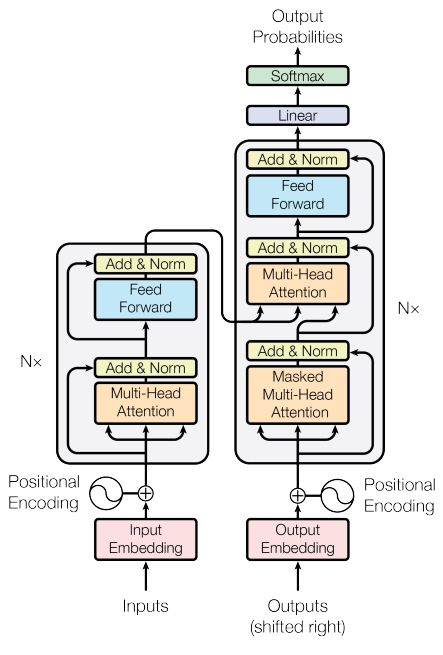
\includegraphics[scale=0.6]{Res/transformers-img1.jpg}
\caption{A arquitetura do modelo \textit{transformer}. Na esquerda, o
codificador. Ele recebe as \textit{embeddings} de entrada, as preprocessa
somando-as com \textit{embeddings} de codificação posicional e envia isso como
entrada para $N$ cabeças de atenção, que enviarão seu resultado para o
decodificador. Na direita, o decodificador. Ele recebe as \textit{embeddings} da
saída anterior ao \textit{token} que se deseja produzir e as preprocessa
somando-as com \textit{embeddings} de codificação posicional e envia isso como
entrada para $N$ cabeças de atenção, que recebe também como entrada os
\textit{embeddings} do codificador. Ao final, o resultado é enviado para uma
camada linear, que transforma a saída em um único vetor que é enviado ara uma
camada \textit{softmax}, que retorna uma distribuição de probabilidades. Imagem
retirada de \cite{vaswani-etal:2017:attention-is-all-you-need}.}
\label{transformers-img1.jpg}
\end{figure}

O mecanismo de atenção do transformer é um pouco diferente e é chamado de
\textit{scaled dot-product attention} (do inglês, atenção de produto escalar
escalado). Assim como na equação \ref{eq:attention}, a atenção é calculada
fazendo uma média ponderada entre os valores atribuídos aos elementos da
sequência. \cite{vaswani-etal:2017:attention-is-all-you-need}, entretanto,
modificam como os pesos de ponderação são calculados. Para isso, eles introduzem
a equação
\begin{equation}
  \texttt{Attention}\paren{Q, K, V}
  =\texttt{softmax}\paren{\dfrac{QK^{T}}{\sqrt{d_k}}}V.
  \label{eq:self-attention}
\end{equation}

Nela, os valores $Q$, $K$ e $V$ são matrizes que representam respectivamente
\textit{consultas}, \textit{chaves} e \textit{valores} (do inglês,
\textit{queries}, \textit{keys} e \textit{values}). Essa função de atenção é
aplicada um número $h$ de vezes na mesma entrada, mas resultando em consultas,
chaves e valores diferentes. Isso pois um tipo de atenção pode relacionar
elementos que sejam das mesmas classes sintáticas e replicar o comportamento de
alguns dos métodos de regras vistos na sessão
\ref{sub:abordagens_baseados_em_regras}, enquanto outras atenções podem
olhar para a semântica de termos relacionados.

Essas $h$ ``cabeças'' de atenção possuem seus resultados concatenados em uma
saída única que pode ser processada pela próxima camada da rede neural. Essa
camada cheia de cabeças recebe, portanto, o nome de atenção multi-cabeça (do
inglês, \textit{multi-head attention}).

\begin{figure}[h]
\centering
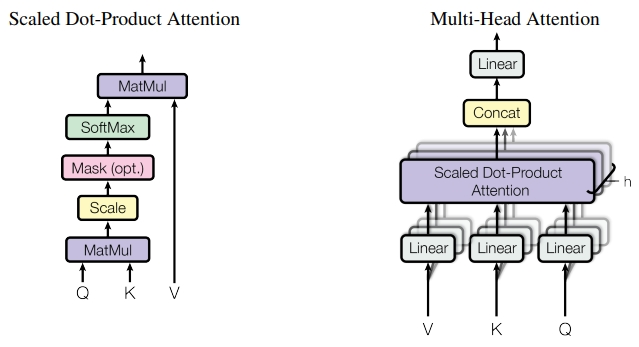
\includegraphics[scale=0.6]{Res/transformers-img2.jpg}
\caption{Na esquerda, a atenção de produto escalar escalado. Na direita, a
atenção multi-cabeça, com várias camadas que podem ser executadas em paralelo.
Imagem retirada de \cite{vaswani-etal:2017:attention-is-all-you-need}.}
\label{transformers-img2.jpg}
\end{figure}



No codificador, $Q$, $K$ e $V$ são todas providas pelo próprio codificador (ou
pela sequência de entrada, no cabeço da primeira camada). Já no decodificador,
os valores de $Q$ e $K$ são providos pelo codificador e os valores $V$ são
criados pelo próprio decodificador com base na sequência esperada de saída.
Dessa forma, a rede presta atenção na sequência de saída, mas levando como base
a sequência de entrada.

Por fim, é importante mencionar que, apesar de resolver o problema do
processamento sequência anteriormente mencionado, os \textit{transformers} criam
um novo problema que é o de não representar adequadamente a característica
sequêncial de suas entradas. Como não se utiliza RNNs, pode-se pensar em um
\textit{transformer} como se fosse uma rede neural completamente conectada
(DNN). Esse tipo de rede não é bom em saber que existe relação entre o elemento
$x_1$ e $x_2$ e que, essa relação é uma métrica com o dobro de valor para $x_1$
e $x_3$. Para dar uma solução parcial a esse problema, os autores propõem uma
codificação posicional que deve ser adicionada à representação original das
palavras. Portanto, o valor da entrada que o modelo realmente recebe é
$x_i+PE(i)$ para a entrada $i$.

O modelo completo é muito mais complexo do que o apresentado aqui e recomenda-se
ao leitor a leitura completa do artigo por
\cite{vaswani-etal:2017:attention-is-all-you-need} caso ele tenha mais interesse
no assunto.

\subsection{BERT}%
\label{sub:bert}

Para finalizar o capítulo, falar-se-á de um dos modelos de redes
\textit{transformers} que é vastamente aplicado em problemas de NLP e que é uma
das bases para o modelo explorado nesse trabalho. Este \textit{transformer} é o
BERT, que é uma sigla para \textit{Bidirectional Encoder Representations from
Transformers} (em tradução livre, ``representações de codificação bidirecional
de \textit{transformers}'')~(\cite{devlin-etal:2018:bert}).

A principal inovação desse modelo é que ele torna o treinamento bidirecional
através de um objetivo de treinamento denominado \textit{masked language model}
(MLM) (do inglês, modelo de linguagem mascarada). Nesse tipo de treinamento,
alguns dos \textit{tokens} da sequência de entrada são aleatoriamente
mascarados (isto é, trocados por um \textit{token} específico \texttt{<MASK>}) e
a tarefa alvo do treinamento é justamente identificar quais eram as palavras
originais, antes de serem mascaradas.

Isso faz com que o modelo possa utilizar o contexto bidirecionalmente, ou seja,
observar as palavras ao redor da palavra alvo para predizê-la. Por exemplo, na
frase ``A roda do meu \texttt{<MASK>} quebrou novamente'', as palavras ``roda''
e ``quebrou'' são importantes para supor que \texttt{<MASK>} corresponde à
palavra ``carro'' ou algum automóvel similar. De forma análoga, o modelo
BERT pode utilizar essas palavras ao redor da palavra mascarada para estimar
qual palavra ela era originalmente.

As aplicações desse modelo são vastas, mas para o escopo deste trabalho, basta
saber que ele pode ser utilizado também na detecção automática de sarcasmo
(\cite{yaghoobian:2021:sarcasm-detection-comparative-study}).
